\chapter{Fundamentals of realistic image synthesis}
\label{ch:2}
In this chapter we briefly revise fundamental theory behind realistic computer generated imagery. Our aim is to synthesize (render) image of a virtual scene. To do this properly, with physical accuracy in mind, we have to find a suitable physical model of light.
\\
\\
If we would like to be absolutely correct, we would have to use quantum optics model. This would lead us to tracing individual photons and interaction with matter on an atomic level, which is completely computationally unfeasible. Nevertheless when it comes to computer graphics even a simplified ray optics model can handle majority of the phenomena we are interested in. This model assumes that light travels in straight lines, at infinite speed and the only things that might happen to it are emission, absorption, reflection, and transmission. Using this model we will be unable to simulate phenomena such as diffraction (for example chromatic aberration), polarization and other similar effects depending on light wavelengths and polarity.
\\
\\
When the suitable light model is chosen, we should define some numerical quantities we can compute with. In the next section we will start with radiometry quantities and inspect problem of light interaction with surfaces. This gives us enough fundaments to formulate rendering equation. We continue with light interaction with participating media, which leads us to extended rendering equation. Algorithms mentioned in the next chapters are based on this theory and they present various methods solving this complex equation.
\\
\\
%have to add here page
%\clearpage{}
\section{Radiometry}

Radiometry is set of techniques for measuring different kinds of electromagnetic radiation such as light. We could have used a photometry, which on the other hand measures the response of a human eye to visible light. This basically corresponds to measurements retrieved using radiometry and weighted with an eye response function. For the purposes of this thesis we will use radiometric quantities, because corresponding photometric quantities can be easily derived.

\subsection{Radiometric quantities}
\begin{equation}
\phi=\frac{dQ}{dt}\;\;[W=J.s^{-1}]
\end{equation}
\bd{Radiant flux}, also known as radiant power, denoted as $\phi$. This quantity corresponds to the light power mentioned on the light bulbs in Watts.
%prehodit vety a pridat 
Where Q [J] denotes radiant energy, which describes how much energy (amount of photons times their energy) is presented in a given area at a point in time. This leads us to flux definition as  amount of radiant energy going through a location over time , alternatively speaking how fast is the change of the amount of the photons in a specified location. 
\line(1,0){450}
\begin{equation}
E(x)=\frac{d\phi(x)}{dA}\;\;[W.m^{-2}]
\end{equation}
\bd{Irradiance}, also known as flux density, denoted as \ita{E(x).} The irradiance at a point \ita{x} on the surface \ita{S,} can be expressed as an amount of incident flux to differential area at a given time.

\noindent{\line(1,0){450}}
\begin{equation}
\label{eg:rd}
L(x,\omega)=\frac{d\phi(x)}{cos\theta dAd \omega}\;\;[W.m^{-2}.sr^{-1}]
\end{equation}
\bd{Radiance} is probably the most important quantity. Denoted as $L(x,\omega)$, where x is a point of interest and $\omega$ is a differential angle coming in a given direction, also known as solid angle.Radiance expresses how much flux is coming from a differential direction $d\omega$ onto a differential surface $dA$. The $cos\theta$ factor compensates the shortening amount of irradiance on the surface with growing $\theta$\footnote{The meaning of $\theta$ is $cos(\theta)=(\vec{n}.\vec{\omega})$, where $\vec{n}$ is surface normal at a point of interest (x) and $\vec{\omega}$ is a direction vector we want to compute radiance for.}, while the level of illumination is maintained. This is the quantity, which has to be gathered for every pixel in the rendered image.

\subsection{Relationships between quantities}
In order to render our image we have to compute radiance coming from the scene through every pixel of the virtual camera sensor. From the table \ref{tab:title} you can see that radiance units are Watts per square meter per steradian\footnote{Steradian is unit of a solid angle.}. According to the units of the remaining radiometry quantities we should be able to derive them using integration.\\
\\

\begin {table}[H]
\centering
\begin{tabular}{lll}
\hline
Radiant energy&$Q$&[J]\\
Radiant flux&$\phi$&[W]\\ 
Irradiance&$E$&[$W.m^{-2}$]\\ 
Radiance&$L$& [$W.m^{-2}.sr^{-1}$]\\
\hline
\end{tabular}
\caption {Table summary of the radiometric quantities.} \label{tab:title} 
\end{table}

\noindent{
If we integrate incoming radiance over a hemisphere denoted as $\Omega$ in a given point \ita{x} \\we get equation \ref{eq:IrradianceInt}. Notice a $-\omega$ in the equation, this is caused by the fact that $\Omega$ usually refers to hemisphere consisting of outgoing solid angles. But when computing irradiance we are interested in the incoming radiance.
}

\begin{equation}
E(x)=\int_{\Omega}L(x,-\vec\omega)*cos(\theta)d\vec\omega
\label{eq:IrradianceInt} 
\end{equation}
\noindent{
To get flux from radiance, we will have to perform two integration steps. We will have to integrate radiance over a hemisphere in every differential surface, which belongs\\ to the surface we are interested in. This is precisely written in the equation \ref{eq:fluxInt}.
}
\begin{equation}
\phi=\int_{A}\int_{\Omega}L(x,\vec\omega)*cos(\theta)d\vec\omega dA
\label{eq:fluxInt} 
\end{equation}

\clearpage{}
\section{Surface interaction}
Using ray optics model, light can interact with object in only four ways. It can be created by the object, which is referred as an emission. On the other way it can be partially or fully absorbed, reflected or refracted in the same time.
\\
\\
As was mentioned in the beginning of this chapter, it's almost impossible to simulate these light interactions in large scenes using light interaction on a molecular level. Currently the most used scene representation is probably an object boundary representation\footnote{Consisting of a finite set of triangles, quadrangles and other n-gons.}. Unfortunately the microscopic structure of the object plays a huge role in the light interaction as can be seen on the fig  \ref{fig:METAL} and would again result in an immense complexity if represented using triangles. To cope with this problem we usually model the corse object shapes using the boundary representation and we call the microscopic behavior "the material behavior". To model the material behavior we use the BRDF function.

\myFigure{0.7}{images/temp}{Brushed, unbrushed, diffuse BRDF metal surface.}{This is an example of the same material (aluminum metal) with different surface texture. From left to right brushed, polished and surface after abrasive blasting. Below each image you can see corresponding schematic BRDF function}{fig:METAL}
%In this image there will be schema of the brdf function different lobes, incoming and outgoing dirrections Theta angle normal .....
\subsection{BRDF}
The \ita{bidirectional reflectance distribution function} describes what is the probability that an incoming light from a given incoming direction will reflect to a given outcoming direction from the given surface. As stated before we can define the BRDF function as:
\begin{equation}
f(\omega_{i},x,\omega_{o})=\frac{dL_{o}(x,\omega_{o})}{dE(x,\omega_{i})}=\frac{L(x,\omega_{o})}{L_{i}(x,\omega_{i})*cos(\theta_{i})d\omega_{i}}
\end{equation}

\noindent{
To formulate the BRDF function more precisely we should define it's properties:
}
 \begin{enumerate}
\item \bd{Function domain:}\\
For a given surface point \ita{x} the BRDF is four dimensional function. Two dimensions for the incoming direction and two for the outgoing direction.

\item \bd{Value range:}\\
BRDF can gain any positive value. For example using constant BRDF functions we can model diffuse materials.

\item \bd{Reciprocity:}\\
The BRDF value stays the same if we interchange incoming and outgoing direction. This is a the very fundamental property many global illumination algorithms rely on. Thanks to this behavior we can gather or shoot light energy using the same BRDF functions and all light interactions remain the same. 

\item \bd{Linearity:}\\
It's a linear function, thus it is not dependent on irradiance from other directions. To get total reflected radiance in the given direction $\omega_{o}$ and given point we get an equation \ref{eq:brdfrad}.
 \begin{equation}
L_{o}(\vec\omega_{o})=\int_{\Omega}L_{i}(\vec\omega_{i})*f_{r}(\vec\omega_{i},\vec\omega_{O})*cos(\theta)d\vec\omega
\label{eq:brdfrad} 
\end{equation}

\item \bd{Energy conservation:}\\
Total reflected energy to all directions is smaller or equal to the total irradiance in any given point. This ensures that an object can't reflect more light than it receives. 

\end{enumerate}
\clearpage{}
\subsection{Rendering equation}
We have successfully defined the quantities we want to compute and models we want to use for the light surface interaction. What we want to achieve is to distribute the light energy in the scene and compute the energy fraction which reaches our image pixels.
\\
\\
To describe the energetic equilibrial state in the scene\footnote{This refers to the light distribution in the scene.} we use rendering equation \ref{eq:rend}. As you can see it closely resembles the equation \ref{eq:brdfrad}. The main difference between these two equations is the fact that the unknown radiance \footnote{Both $L(r(x,\omega_i),-\omega_{i})$ and $L(x,\omega_{o})$ are unknown.} is on both sides of the equation and that instead of the local radiance $L(x,\omega_{o})$ we want to trace a ray in a direction $\omega_{i}$ to the scene and compute the radiance in closest ray surface intersection $L(r(x,\omega_i),-\omega_{i})$.
\\
\\
\begin{equation}
L(x,\omega_{o})=\int_{\Omega}L(r(x,\omega_i),-\omega_{i})*f(\omega_{i},x,\omega_{o})*cos(\theta_{i})d\omega_{i}
\label{eq:rend}
\end{equation}
\begin{equation}
\overbrace{L(x,\omega_{o})}^\text{outgoing}=\underbrace{L_{e}(x,\omega_{o})}_\text{emited}+\underbrace{\int_{\Omega}L(r(x,\omega_i),-\omega_{i})*f(\omega_{i},x,\omega_{o})*cos(\theta_{i})d\omega_{i}}_\text{reflected}
\label{eq:rendem}
\end{equation}
\noindent{
The equation \ref{eq:rend} can deal with light reflection, refraction and absorption. To consider the light emitting objects in our scene we have to introduce an emitted radiance \footnote{$L_{e}(x,\omega_{o})$ } into the equation. Which result in eq \ref{eq:rendem}. To get an actual image of our scene $L(x,\omega_{o})$ (outgoing radiance) has to be computed for every image pixel.
}

\clearpage{}
\section{Volume interaction}
\label{sec:VOLINTER}
By now we have assumed that radiance is conserved along its ray path between surfaces. It's time to consider participating media interaction in our computation. To do this we should define some properties, which can be used to model and describe different types of volumetric phonomenons.

\begin{description}
\item[$\boldsymbol{\kappa_{a}\; [m^-1]}$ - \bd{Absorption coefficient}] is equal to the probability that a photon gets absorbed in volumetric media, per unit of distance along it's flight direction. In other words what is the probability that the photon will hit molecule and gets absorbed\footnote{Absorbed equals to transformation of photon energy to other kinds of energy, such as heat radiation.}. This leads to radiance reduction.

\item[$\boldsymbol{\kappa_{s}\; [m^-1]}$ - \bd{Scattering coefficient }] is equal to probability that the photon will by scattered\footnote{Scattering is process when radiation is forced to deviate from it's straight path to other directions.}, per unit of distance along it's flight direction. This again leads to radiance reduction in the original photon flow direction, but also to radiance propagation into other directions.

\item[$\boldsymbol{\kappa_{t}\; [m^-1]}$ - \bd{Extinction coefficient}] is a summation of the two preceding properties. It equals to probability that the photon will collide with the particles in the media\footnote{The probability that it gets scattered or absorbed.}, which gives us following relationship: $\kappa_{t}=\kappa_{a}+\kappa_{s}$.

\end{description}
\noindent{
We distinguish four different types of interaction events, which have got a lot in common with previously defined coefficients:
}
 \begin{enumerate}
 \item \bd{Absorption:}\\
$\boldsymbol{\kappa_{a}}$ gives us the probability of absorption. To evaluate an effect to the incident radiance we simply subtract proportional part of it as follows:
\begin{equation}
 	dL_{a}(x,\omega_{0})=-\kappa_a(x)*L(x,\omega_{0})dx
 \end{equation}

\item \bd{Volume emission:}\\
To simulate any light emitting volumetric phenomenons like fire or aurora, we have to add some energy to the ray going through this media. The emission contribution to the radiance equals to:
\begin{equation}
 	dL(x,\omega_{0})=\kappa_a(x)*L_{e}(x,\omega_{0})dx
 \end{equation}

\item \bd{Out-scattering:}\\
The radiance going through the media can get scatter, thus the original energy flow might participate into many new directions. The probability that this will happen is described by $\boldsymbol{\kappa_{s}}$, so the radiance loss can be describeded as:
\begin{equation}
	dL(x,\omega_{0})=-\kappa_s(x)*L(x,\omega_{0})dx 
\end{equation}

\item \bd{In-scattering:}\\
To sum the total radiance in a given point in the media we have to cope with the consequences of out-scattering from the surrounding media. To do it we have to integrate incoming radiance to a point in the space from all possible directions and weight it with the probability that the scattering from these directions will happen $\boldsymbol{\kappa_{s}}$. This leads us to eq. \ref{eq:INSCATT}. The $p(x,\omega_{0},\omega_{i})$ is phase function, which will be described further in the next section \ref{subsec:PHASE}.
\begin{equation}
\label{eq:INSCATT}
%podle Sloupovych prednasek
 	%dL_{i}(x,\omega_{0})=\frac{\kappa_t(x)}{4\pi}*\int_{\Omega}L(x,\omega_{i})p(x,\omega_{0},\omega_{i})d\omega_{i}
	%podle Jarosze
	dL_{i}(x,\omega_{0})=\int_{\Omega}L(x,\omega_{i})p(x,\omega_{0},\omega_{i})d\omega_{i}
 \end{equation}
 
\end{enumerate}

\noindent{
For better understanding take a look on the picture fig\ref{fig:EAIO}. Since all the above equations considered only a differential volume we will have to extend it in section \ref{sec:EXTREND}.
}
\myFigure{0.35}{images/temp}{Volume absorption, emission, in and out-scattering.}{This fig can be helpful to understand how each of the absorption, emission, in and out-scattering events affects the radiance.}{fig:EAIO}

\clearpage{}
\subsection{Phase functions}
\label{subsec:PHASE}
To model a light interaction on a molecular level, we use phase functions\footnote{Analogically to the BRDF functions, which model light surface interaction on microscopical level and simulate different surface materials.}, which can be used to model different volumetric media types. It describes the probability of scattering light from incoming direction $\omega_{i}$ to the outgoing direction $\omega_{o}$.
\\
\\
Phase function has got these useful properties:
 \begin{enumerate}
\item \bd{Function domain:}\\
Is the same as in the case of the BRDF function. For the given point in the space it is four dimensional function. Two dimensions for incoming and to for the outgoing direction.
\item \bd{Value range:}\\
Greater than zero and it's very useful to normalize phase function values so that:
\begin{equation}
\int_{\Omega\text{4}\pi}p(\omega_{i},x,\omega_{i})=1
\end{equation}
This way we can be sure that the energy will be conserved.
\item \bd{Reciprocity:}\\
The phase function value stays the same if we interchange incoming and outgoing direction.
\item \bd{Conservation:}\\
The incoming radiance is always greater or equal to the sum of the distributed energy into all directions.
\end{enumerate}
\noindent{
The phase function depends heavily on the ratio between the light wavelength and particle size of the volumetric media. Since we are interested mainly in the visible light spectra, we can narrow the dependency on the particle size. Fig \ref{fig:PARTSIZE} shows different phase function approximations, depending on the growing particle size. As you can see it is extremely difficult to describe this complex behavior globally in one analytical model function. Thus multiple models are used in practice, each one is suitable only for some media types. 
}
\myFigure{0.35}{images/temp.jpg}{Phase function dependency with fixed light wavelength on growing particle sizes.}{Phase function dependency with fixed light wavelength on growing particle sizes. More details about the functions are in the sections \ref{lab:REY},\ref{lab:HEN} ,\ref{lab:MIE} . }{fig:PARTSIZE} 
%\clearpage{}
\subsubsection{Heney-Greenstein phase function}
This phase function can nicely approximate both forward and backward light scattering behaviors, modifying only one variable \ita{g.} The function is defined as:
\begin{equation}
\label{eq:HENEYGREEN}
HG(\theta)=\frac{1-g^{2}}{4\pi(1+g^{2}-2gcos(\theta))^{frac{3}{2}}}
\end{equation}
Thanks to it's flexibility and low computational complexity it's widely used to simulate dust, smoke even water light behavior. The fig \ref{fig:HG2} demonstrates how is the ratio between forward and backward scattering dependent on the \ita{g} value, while fig \ref{fig:HG3} shows a 3D shape of forward scattering phase function.

\label{lab:HEN}
\begin{minipage}{\linewidth}
      \begin{minipage}{0.45\linewidth}
          \begin{figure}[H]
              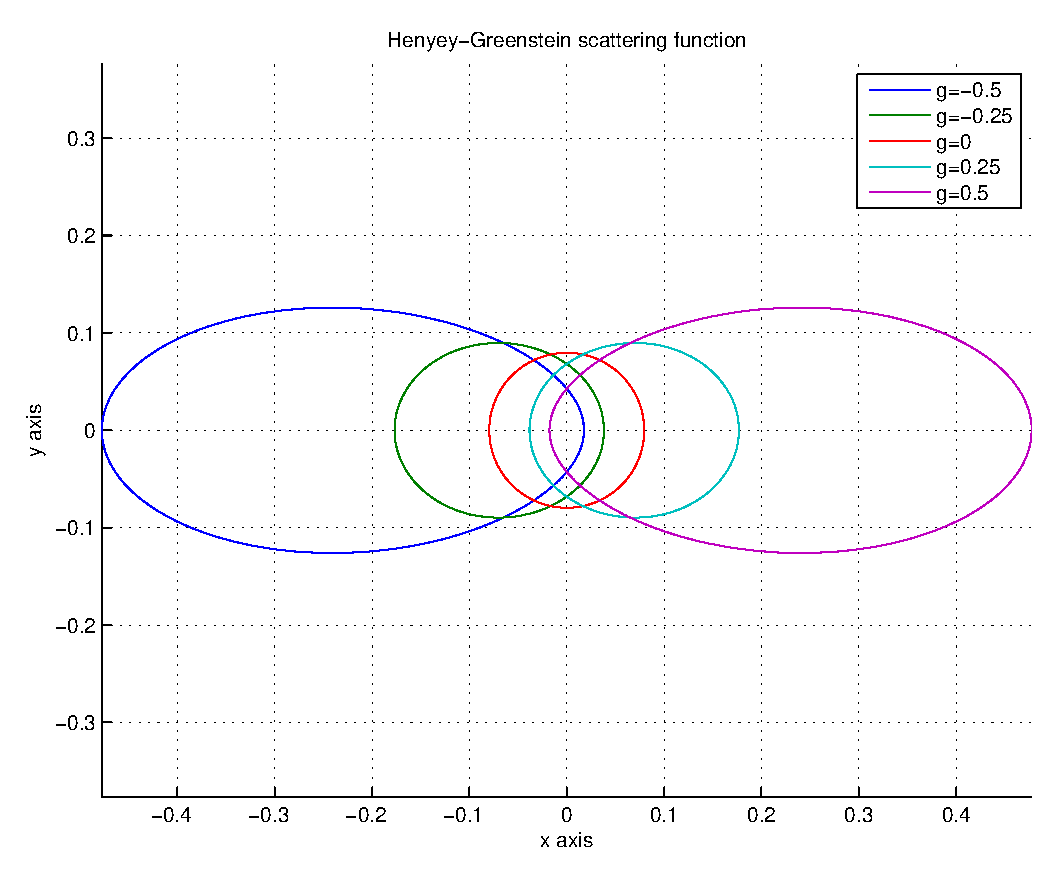
\includegraphics[width=\linewidth]{02_Chap2/Figures/heneygreenstein2dgraph}
              \captionsetup{width=\linewidth}
              \caption[2D plot of Plot of Heney-Greenstein phase function.]{Plot of Heney-Greenstein phase function with different g coefficients. For g\textless0 the function represents backscattering media, for g=0 isometric scattering and for g\textgreater0 growing forward scattering tendencies.}\label{fig:HG2}
          \end{figure}
      \end{minipage}
      \hspace{0.05\linewidth}
      \begin{minipage}{0.45\linewidth}
          \begin{figure}[H]
              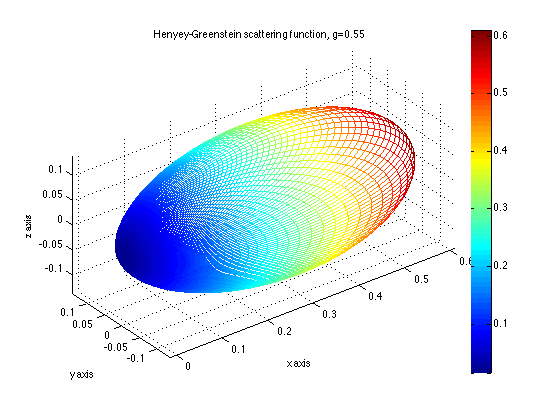
\includegraphics[width=\linewidth]{images/hg3d}
              \captionsetup{width=\linewidth}
              \caption[3D plot Heney-Greenstein]{3D plot of Heney-Greenstein phase function with scattering coefficient set to 0.55, which results in moderate forward scattering. }\label{fig:HG3}
          \end{figure}
      \end{minipage}
  \end{minipage}
\clearpage{}

\subsubsection{Rayleigh Scattering}
\label{lab:REY}
Rayleigh scattering models interaction between electromagnetic radiation and particles, which should be much smaller than the radiation wavelength. Since it can model different wavelengths, polarizations and particle sizes, it is a widely used in scientific computation and computer graphics. It's an ideal model for light atmosphere interaction, because it describes the scattering coefficient dependency on light wavelength as eq. \ref{eq:RFRA}. The effects it has on the atmosphere appearance can be seen on fig \ref{fig:REYLIGHSUNSET}.
\begin{equation}
\label{eq:RFRA}
\kappa_{s}=\frac{1}{\lambda^{4}} 
\end{equation}
The original equation \ref{eq:RAYLEIGH} is really general, $I_0$ is incoming light intensity, $\sigma$ is light wavelength, $n$ is refractive index of particles, $R$ is distance to particle and $d$ is the diameter of the particle. 
\begin{equation}
\label{eq:RAYLEIGH}
I=I_{0}\frac{1+cos^{2}(\theta))}{2R^2}*\left(\frac{2\pi}{\lambda}\right)^{4}*\left(\frac{n^{2}-1}{n^{2}+2}\right)^2*\left(\frac{d}{2}\right)^6
\end{equation}
\noindent{
Since many of these coefficients, can be considered constant in the media we can put them into scattering coefficient $\sigma_{s}$. Resulting polar plot is in the fig \ref{fig:REYLIGH} and the phase function is following:
}
\begin{equation}
\label{eq:RAYLEIGH2}
R(\theta)=\frac{3}{16\pi}(1+cos^{2}(\theta)); \text{\;\;\;\;} \sigma_{s}=\frac{2\pi^{5}*d^{6}}{\lambda^{4}*3}*\left(\frac{n^{2}-1}{n^{2}+2}\right)^2
\end{equation}

\label{lab:HEN}
\begin{minipage}{\linewidth}
      \begin{minipage}{0.45\linewidth}
          \begin{figure}[H]
              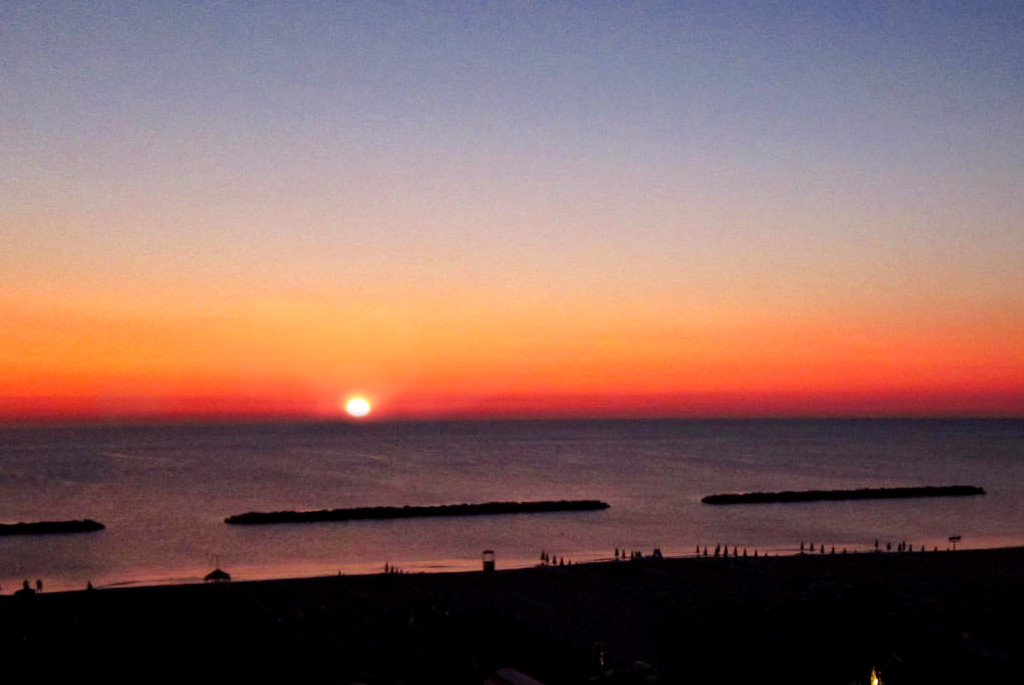
\includegraphics[width=\linewidth]{images/sunsetbeach.jpg}
              \captionsetup{width=\linewidth}
              \caption[Sunset atmospherical behavior.]{Because shorter wavelengths are scattered more, the red color light spectra dominates on the horizon, where the light path through the atmosphere is longest.}\label{fig:REYLIGHSUNSET}
          \end{figure}
      \end{minipage}
      \hspace{0.05\linewidth}
      \begin{minipage}{0.45\linewidth}
          \begin{figure}[H]
              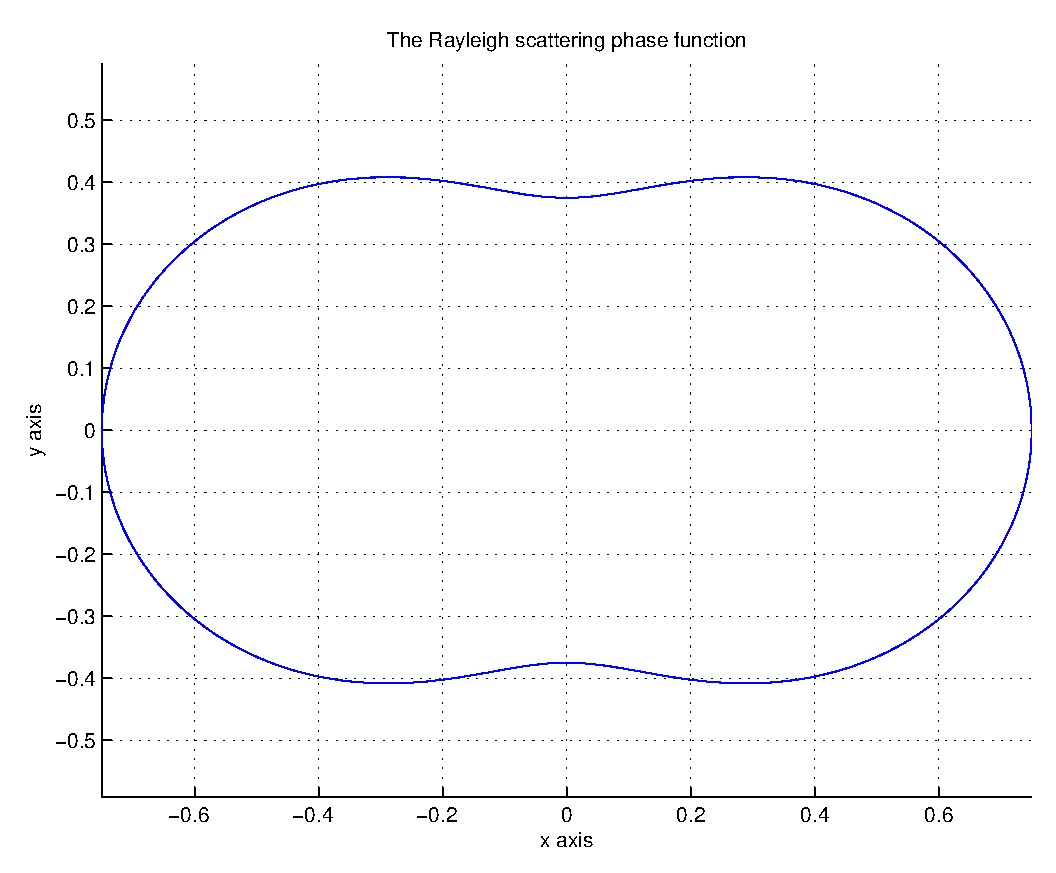
\includegraphics[width=\linewidth]{images/reyleigh2dgraph}
              \captionsetup{width=\linewidth}
              \caption[2D polar plot of Rayleigh scattering function.]{2D polar plot of  function Rayleigh scattering function.}\label{fig:REYLIGH}
          \end{figure}
      \end{minipage}
  \end{minipage}


\subsubsection{MIE scattering}
\label{lab:MIE}
Probably the most elaborate model of all mentioned. It's based on the theory of Lorenz–Mie solution to Maxwell's equations. It is used to simulate light interaction with particles, which size is approximately equal to the light wavelength. These properties make it an ideal candidate for light water droplet interaction simulations such as cloud, mist, rain lighting. Since it is wavelength dependent it can be used to simulate effects such as rainbows or coronas.
\\
\\
Unfortunately it's quite computation costly \footnote{Approximation method's do exist and will be presented in the chapter \ref{chap:IMPLEM}.}. It's usually evaluated once for the whole $\theta$ domain\footnote{We usually assume symmetric behavior along an incoming light direction, which results in $<0;\pi>$ interval for $\theta$.} in the pre computation phase and stored to lookup table. Sample polar plot of the function can be seen on the fig \ref{fig:MIEPLOT}. Notice the major forward peak, which carries almost $50\%$ of the incoming energy\footnote{Even though it might not be absolutely evident, from the logarithmic scale polar plot.}, this property makes it even more challenging for an efficient importance sampling techniques, because the side scattering might be easily omitted, leading to loss of rainbow like effects.

\myFigure{0.5}{images/r10PerpPolarLogA.png}{MIE scattering polar plot of red light with water droplet interaction. Source \cite{MIEPLOT}}{Polar diagram of scattering of red light (wavelength 0.65 $\mu$m, perpendicular polarization) from a water droplet of r = 10 $\mu$. Source \cite{MIEPLOT}. }{fig:MIEPLOT} 

\clearpage{}
\section{Volume and surface interaction}
\label{sec:EXTREND}
In order to properly simulate light transport in the scenes containing both surfaces and volumetrically active media, few adjustments to the rendering equation have to be made.
\\
\\
First of all, the participating media can add radiance to the pixel, because of both emission and in-scattering. On the other hand the surface radiance contribution can be attenuated, because of the media absorption and out-scattering. To accommodate these effects into rendering equation, we have to extend the volume interaction theory  from differential volume slice (sec. \ref{sec:VOLINTER}) to brother volume section.

\subsection{Radiance losses}
The loss of radiance caused by out-scattering and absorption is very often called transmittance. The equation for differential volume looks like this:
 \begin{equation}
\label{eq:EXTRANS}
dL(x,\omega)=-\kappa_a(x)*L(x,\omega)dx-\kappa_s(x)*L(x,\omega)dx =-\kappa_t(x)*L(x,\omega)dx
\end{equation}
\noindent{
To integrate overall loss over a longer segments of the media we have to compute its \bd{optical thickness} as fallows:
}
\begin{equation}
 	\int_{x_{0}}^{x}\kappa_t(x_{v})dv
 \end{equation}
 \noindent{
 where the $x_{0}\text{ and }x$ are the end points of the media section we are interested in. According to the \ita{Beer–Lambert law} \cite{bouguer1729essai} we can now evaluate the total transmittance between two points in the media as follows:
 \begin{equation}
 \label{eq:TAU}
   \tau(x_0,x)=e^{-\int_{x_{0}}^{x}\kappa_t(v)dv};
 \end{equation}
Now we can express the overall radiance loss as:
\begin{equation}
L(x,\omega)=L(x_0,\omega)\tau(x_0,x)
\end{equation}

\clearpage{}
\subsection{Radiance gains}
In the terms of radiance gains the equations are quite straight forward. The only thing we have to do is to weight the gain with appropriate probability and attenuate it with corresponding transmittance. This way we get following equation, which express the radiance gain over a given volumetric path segment:
\begin{equation}
L(x,\omega)= \int_{x_{0}}^{x}
    \underbrace{
      \tau(x_{0},x_{v})\kappa_{a}(v)L_{e}(x,\omega)
     }_{\text{attenuated emitted radiance}}
    +
    \underbrace{
       \tau(x_{0},x_{v})\kappa_{s}(v)L_{i}(x_{v},\omega)
    }_{\text{attenuated in-scattered radiance}}
    dv
\end{equation}

\subsection{Extended rendering equation}
Now we have all the necessary elements to put together an extended rendering equation for rendering both surfaces and volumetrically active media. Eq. \ref{eq:VOLRENDEQ} is known as radiative transfer equation \cite{chandrasekhar1960radiative}. By extending this equation from differential volume to the fully integral form we get eq. \ref{eq:EXTINTFORM}.

\begin{equation}
\label{eq:VOLRENDEQ}
dL(x,\omega)=\overbrace{\underbrace{{-\kappa_{a}L(x,\omega)} }_{absorption}\underbrace{-\kappa_{s}L(x,\omega)} _{out-scattering} }^\text{dissipation loss} \overbrace{\underbrace{{+\kappa_{a}L_{e}(x,\omega)} }_{emission}\underbrace{+\kappa_{s}L_{i}(x,\omega)} _{in-scattering} }^\text{gain}dx
 \end{equation}
 
 \begin{equation}
 \label{eq:EXTINTFORM}
 L(x,\omega)=\overbrace{\underbrace{L(x_{0},\omega)}_{\text{surface radiance}}*\underbrace{\tau(x_{0},x) }_{\text{transmittance}}}^{\text{attenuated surface radiance}}+
\overbrace{
  \int_{x_{0}}^{x}
    \underbrace{
      \tau(x_{0},x_{v})\kappa_{a}(v)L_{e}(x,\omega)
     }_{\text{attenuated emitted radiance}}
    +
    \underbrace{
       \tau(x_{0},x_{v})\kappa_{s}(v)L_{i}(x_{v},\omega)
    }_{\text{attenuated inscattered radiance}}
    dv
}^{\text{accumulation of radiance gain}}
 \end{equation} 

\clearpage{}
\section{Volume representation}
We have got many options for volume representation in computer graphics. Rather than representing individual particles\footnote{Even if we want to render large amounts of "particles" we usually might choose to render them as a point cloud where every particle has got one pixel size, this representation is not based on any physical prerequisites, though might serve well in many scenarios.} we usually use larger volumes of space using quantization or some kind of bounding volume representation.

\begin{itemize}
\item \bd{Particle representation}
This representation is widely used in games and movies, for phenomenons like sand, dust. The main advantage is that this representation fits nicely into rasterization pipeline, where each point can be rendered out as a semitransparent point or patch. 
\\
\\
Though it is not very suitable representation for raytracing, because it is really hard to ray-trace something infinitely small without aliasing artifacts. For raytracing one can estimate a volume density based on the neighboring particles. To perform efficiently neighborhood queries an acceleration structure would have to be build upon these points.

\item \bd{Bounding volume representation}
We can use any type of boundary representations and turn them into volumetrically active objects. The easiest way is to use parametric primitives such as boxes, spheres or cylinders. But efficient algorithms for mesh geometry exist too. This way we can represent just the boundary of the volume quite efficiently and fill it with any type of 3D texture\footnote{Be it parametric or classical image stack texture.} or value to alter it's optical characteristics\footnote{Characteristics like absorption, density etc. Discussed in section \ref{sec::VOLINTER}} to get desired results. See fig \ref{fig:BOUND} for examples.

\myFigure{0.5}{images/juiceVolume.jpg}{Boundary volume representation.}{Left image is glass with juice\footnote{Juice can be viewed as an optically active homogenous volume.}, the volume is bounded by triangle mesh, source \cite{novak12vrls}. On the right we can se a simple procedural box filled with heterogenous fog\footnote{We can apply any procedural function to the density of the media, in this case we have used three octaves of perlin noise.}}{fig:BOUND}

\item \bd{Grid representation}
To have an absolute control over each voxel\footnote{Also known as \ita{volumetric pixel} is a volumetric analogy of pixel in 2D. We can imagine it as an element of regular 3D grid.} values we can use some kind of grid representation. For example fluid simulations or MRI\footnote{MRI stands for \ita{magnetic resonance imagery} very often used in radiology for noninvasive interior medial examination. } data come in a form of regularly spaced 3D grids. To over come a cubic space complexity of this representation more evolved structures, such as octree can be used\footnote{Lately a new industry standard format \cite{OPENVDB} for efficient storage and access of sparse volumetric datasets has been established}.

\begin{minipage}{\linewidth}
      \begin{minipage}{0.45\linewidth}
          \begin{figure}[H]
              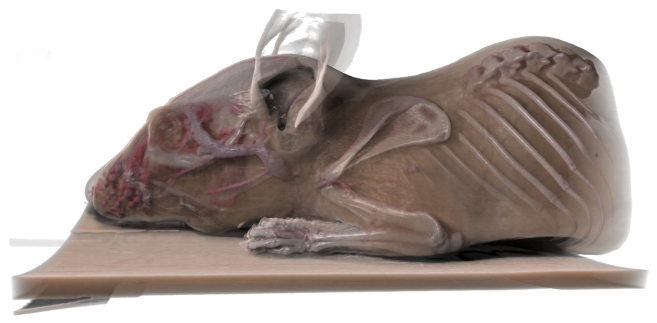
\includegraphics[width=\linewidth]{images/volumerat}
              \captionsetup{width=\linewidth}
              \caption[Volumetric image data example, source \cite{RDR10}.]{Example of a volumetric MRI data set consisting of an image stack. Rendered using Voreen  \cite{RDR10}.}\label{fig:RAT}
          \end{figure}
      \end{minipage}
      \hspace{0.05\linewidth}
      \begin{minipage}{0.45\linewidth}
          \begin{figure}[H]
              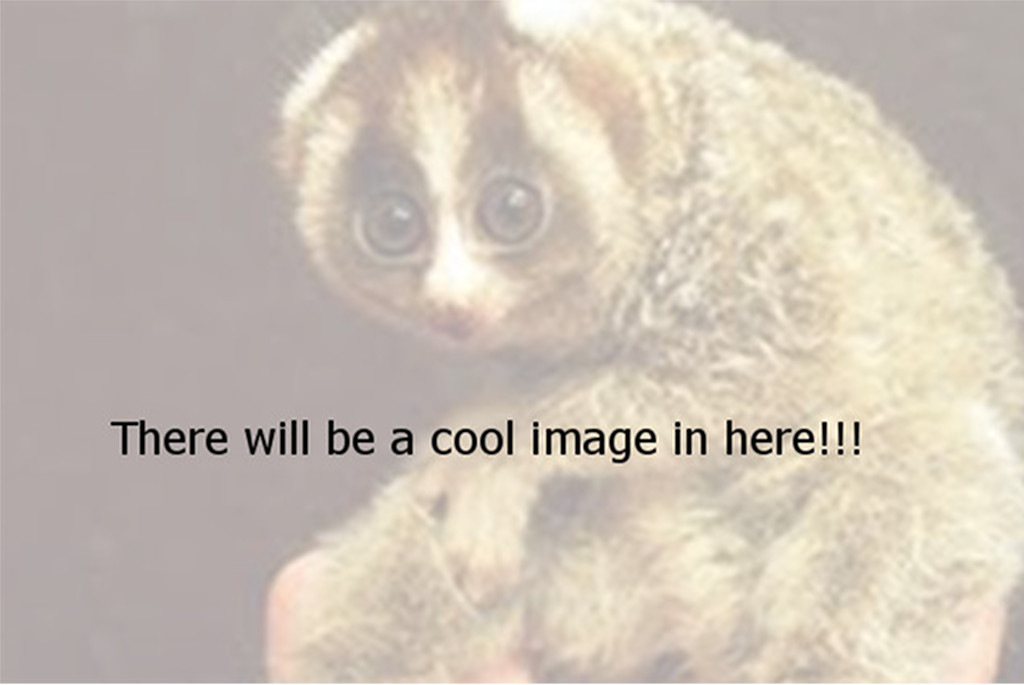
\includegraphics[width=\linewidth]{images/temp}
              \captionsetup{width=\linewidth}
              \caption[Smoke simulation on regular 3D grid.]{Smoke simulation with a simulation grid overlay, each grid cell represents one voxel with different density\footnotemark[1]. }\label{fig:SIMGRID}
          \end{figure}
      \end{minipage}
  \end{minipage}



\end{itemize}

\footnotetext[1]{For the smooth looking results linear interpolation of neighboring values is used.}
%\section{Images and tables}

%\subsection{Images}


